\documentclass[12pt,a4paper]{article}

% --- Packages ---
\usepackage[utf8]{inputenc}
\usepackage[T1]{fontenc}
\usepackage{lmodern}
\usepackage[margin=1in]{geometry}
\usepackage{graphicx}
\usepackage{hyperref}
\usepackage{listings}
\usepackage{xcolor}
\usepackage{booktabs}
\usepackage{enumitem}
\usepackage{amsmath}
\usepackage{float}
\usepackage{caption}
\usepackage{subcaption}
\usepackage{tikz}
\usetikzlibrary{shapes.geometric, arrows.meta, positioning, fit}
\usepackage{fancyhdr}
\usepackage{titlesec}
\usepackage{tocloft}
\usepackage{parskip}

% --- Page Style ---
\pagestyle{fancy}
\fancyhf{}
\fancyhead[L]{\leftmark}
\fancyhead[R]{Lab Surveillance System}
\fancyfoot[C]{\thepage}
\renewcommand{\headrulewidth}{0.4pt}

% --- Code Listing Style ---
\definecolor{codebg}{RGB}{245,245,245}
\definecolor{codegreen}{RGB}{0,128,0}
\definecolor{codegray}{RGB}{128,128,128}
\definecolor{codepurple}{RGB}{128,0,128}
\definecolor{codeblue}{RGB}{0,0,180}

\lstdefinestyle{pythonstyle}{
    backgroundcolor=\color{codebg},
    basicstyle=\ttfamily\footnotesize,
    breaklines=true,
    captionpos=b,
    commentstyle=\color{codegreen},
    keywordstyle=\color{codeblue}\bfseries,
    stringstyle=\color{codepurple},
    numberstyle=\tiny\color{codegray},
    numbers=left,
    numbersep=8pt,
    frame=single,
    rulecolor=\color{codegray},
    language=Python,
    showstringspaces=false,
    tabsize=4,
    morekeywords={self, True, False, None, yield, from, as, with},
}
\lstset{style=pythonstyle}

% --- Title ---
\title{
    \vspace{-1cm}
    \textbf{Qwen Sentinel: AI-Powered Computer Lab Surveillance System} \\[0.5cm]
    \large A Real-Time Video Analytics Platform Using Vision-Language Models \\[1cm]
    \large Technical Report
}
\author{}
\date{February 2026}

\begin{document}

\maketitle
\thispagestyle{empty}

\vfill
\begin{center}
    \textit{Built with Qwen Vision-Language Models, OpenCV, Gradio, and PyTorch}
\end{center}
\vfill

\newpage
\tableofcontents
\newpage

% ============================================================================
\section{Introduction}
% ============================================================================

\subsection{Background and Motivation}

Computer laboratories in educational institutions house expensive equipment and serve as shared workspaces for students and staff. Ensuring that lab rules are followed---such as prohibiting eating, drinking, running, fighting, sleeping, phone usage, and equipment tampering---traditionally requires dedicated human supervision. This is labour-intensive, error-prone, and does not scale.

Recent advances in \textbf{Vision-Language Models (VLMs)} have made it possible to analyse visual data with natural-language understanding. These models can interpret video frames and answer questions about observed activities, opening the door to intelligent, automated surveillance systems that go beyond simple motion detection.

\subsection{Project Overview}

This project, titled \textbf{Qwen Sentinel}, implements a real-time AI-powered surveillance system for computer laboratories. The system:

\begin{itemize}[noitemsep]
    \item Captures video from \textbf{live cameras}, \textbf{RTSP/HTTP streams}, or \textbf{uploaded video files}.
    \item Maintains a \textbf{sliding window frame buffer} and periodically samples frames using configurable strategies.
    \item Sends sampled frames to a \textbf{Qwen Vision-Language Model} for activity detection via natural-language prompting.
    \item Performs a \textbf{two-pass analysis}: first detecting prohibited activities, then localising the offender with bounding-box regression.
    \item Provides a \textbf{web-based dashboard} (Gradio) with live feed display, alert overlays, event logging, and debug tools.
    \item Saves \textbf{evidence snapshots} with annotated bounding boxes for review.
\end{itemize}

\subsection{Scope}

The system targets the following prohibited activities in a lab environment:

\begin{enumerate}[noitemsep]
    \item Running (fast movement across frames)
    \item Fighting or aggressive physical contact
    \item Eating or drinking
    \item Tampering with equipment
    \item Sleeping
    \item Phone usage
\end{enumerate}

% ============================================================================
\section{System Architecture}
% ============================================================================

\subsection{High-Level Architecture}

The system follows a \textbf{multi-threaded producer--consumer architecture} with three main layers:

\begin{figure}[H]
\centering
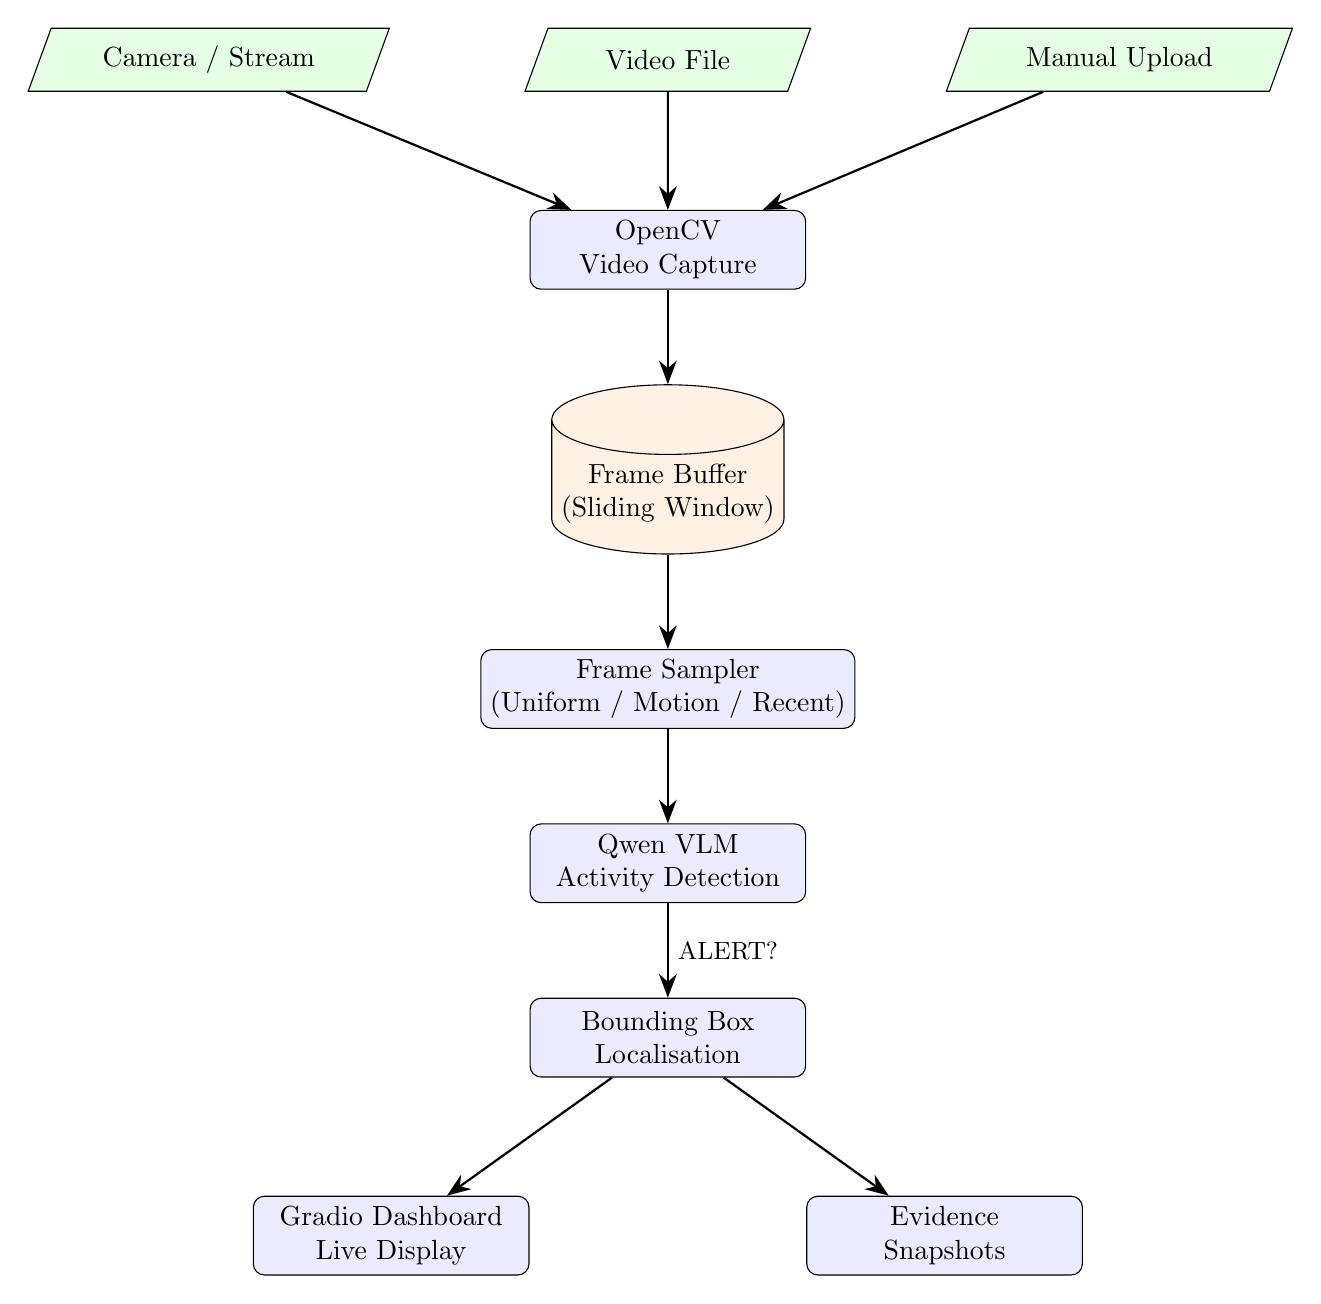
\begin{tikzpicture}[
    node distance=1.2cm and 2cm,
    block/.style={rectangle, draw, rounded corners, minimum width=3.5cm, minimum height=1cm, align=center, fill=blue!8},
    io/.style={trapezium, trapezium left angle=70, trapezium right angle=110, draw, minimum width=2.5cm, minimum height=0.8cm, align=center, fill=green!10},
    data/.style={cylinder, draw, shape border rotate=90, aspect=0.3, minimum height=1.2cm, minimum width=2cm, align=center, fill=orange!10},
    arrow/.style={-{Stealth[length=3mm]}, thick},
]
    % Input Layer
    \node[io] (cam) {Camera / Stream};
    \node[io, right=of cam] (vid) {Video File};
    \node[io, right=of vid] (upload) {Manual Upload};

    % Capture Layer
    \node[block, below=1.5cm of vid] (capture) {OpenCV\\Video Capture};

    % Buffer
    \node[data, below=of capture] (buffer) {Frame Buffer\\(Sliding Window)};

    % Processing
    \node[block, below=of buffer] (sampler) {Frame Sampler\\(Uniform / Motion / Recent)};
    \node[block, below=of sampler] (ai) {Qwen VLM\\Activity Detection};
    \node[block, below=of ai] (bbox) {Bounding Box\\Localisation};

    % Output
    \node[block, below left=1.5cm and 0cm of bbox] (display) {Gradio Dashboard\\Live Display};
    \node[block, below right=1.5cm and 0cm of bbox] (evidence) {Evidence\\Snapshots};

    % Arrows
    \draw[arrow] (cam) -- (capture);
    \draw[arrow] (vid) -- (capture);
    \draw[arrow] (upload) -- (capture);
    \draw[arrow] (capture) -- (buffer);
    \draw[arrow] (buffer) -- (sampler);
    \draw[arrow] (sampler) -- (ai);
    \draw[arrow] (ai) -- node[right, font=\small] {ALERT?} (bbox);
    \draw[arrow] (bbox) -- (display);
    \draw[arrow] (bbox) -- (evidence);
\end{tikzpicture}
\caption{High-level system architecture of Qwen Sentinel.}
\label{fig:architecture}
\end{figure}

\subsection{Module Structure}

The codebase is organised into two main Python modules:

\begin{table}[H]
\centering
\caption{Project file structure.}
\label{tab:files}
\begin{tabular}{@{}lp{9cm}@{}}
\toprule
\textbf{File / Directory} & \textbf{Description} \\
\midrule
\texttt{src/app.py} & Main application: UI, video capture, frame sampling, AI orchestration, display rendering, event logging (1107 lines). \\
\texttt{src/backend.py} & AI backend: model loading, inference pipeline using HuggingFace Transformers and Qwen VL utilities (292 lines). \\
\texttt{requirements.txt} & Python dependencies (77 packages). \\
\texttt{install.ps1} & PowerShell installation script for PyTorch (CUDA), Transformers, and optional GGUF/llama-cpp-python support. \\
\texttt{evidence\_snapshots/} & Directory for saved alert evidence images. \\
\bottomrule
\end{tabular}
\end{table}

\subsection{Threading Model}

The system uses a \textbf{multi-threaded design} to decouple frame capture from AI inference:

\begin{itemize}
    \item \textbf{Main Thread (Gradio Generator):} Captures frames from the video source, appends them to a shared frame buffer, renders display frames with overlays, and yields UI updates to the Gradio frontend.
    \item \textbf{AI Worker Thread:} A long-lived daemon thread that waits on a \texttt{threading.Event}. When triggered by the main thread (based on a configurable time interval), it takes a snapshot of the frame buffer and runs AI analysis. Results are written to shared state under a lock.
    \item \textbf{Synchronisation:} Three locks protect shared data---\texttt{buffer\_lock} for the frame deque, \texttt{state\_lock} for AI results, and \texttt{log\_lock} for log histories.
\end{itemize}

% ============================================================================
\section{AI Backend}
% ============================================================================

\subsection{Supported Models}

The system supports multiple \textbf{Qwen Vision-Language Models} from the Qwen family, loaded via HuggingFace Transformers:

\begin{table}[H]
\centering
\caption{Supported Qwen VL models.}
\label{tab:models}
\begin{tabular}{@{}ll@{}}
\toprule
\textbf{Model Name} & \textbf{HuggingFace Model ID} \\
\midrule
Qwen2-VL-2B-Instruct & \texttt{Qwen/Qwen2-VL-2B-Instruct} \\
Qwen2-VL-7B-Instruct & \texttt{Qwen/Qwen2-VL-7B-Instruct} \\
Qwen2.5-VL-3B-Instruct & \texttt{Qwen/Qwen2.5-VL-3B-Instruct} \\
Qwen2.5-VL-7B-Instruct & \texttt{Qwen/Qwen2.5-VL-7B-Instruct} \\
Qwen3-VL-2B-Instruct & \texttt{Qwen/Qwen3-VL-2B-Instruct} \\
Qwen3-VL-4B-Instruct & \texttt{Qwen/Qwen3-VL-4B-Instruct} \\
Qwen3-VL-8B-Instruct & \texttt{Qwen/Qwen3-VL-8B-Instruct} \\
FP8 variants & FP8-quantised versions of Qwen3-VL models \\
\bottomrule
\end{tabular}
\end{table}

\subsection{Model Loading Pipeline}

The model loading process in \texttt{backend.py} performs the following steps:

\begin{enumerate}
    \item \textbf{Cache Configuration:} The HuggingFace cache directory is configured to reside within the project directory (\texttt{.hf\_cache/}) to keep downloads self-contained. Environment variables \texttt{HF\_HOME}, \texttt{HF\_HUB\_CACHE}, and \texttt{TRANSFORMERS\_CACHE} are set accordingly.
    \item \textbf{Cleanup:} If a model is already loaded, the previous model and processor are deleted, and GPU memory is freed via \texttt{gc.collect()} and \texttt{torch.cuda.empty\_cache()}.
    \item \textbf{Quantisation (Optional):} If 4-bit quantisation is enabled, a \texttt{BitsAndBytesConfig} is created with NF4 quantisation type and \texttt{bfloat16} compute dtype. This reduces VRAM usage significantly.
    \item \textbf{Processor Loading:} The model's tokenizer and image processor are loaded via \texttt{AutoProcessor.from\_pretrained()}.
    \item \textbf{Model Loading:} The model itself is loaded via \texttt{AutoModelForImageTextToText.from\_pretrained()} with automatic device mapping (\texttt{device\_map="auto"}) and automatic dtype selection.
\end{enumerate}

\subsection{Inference Pipeline}

The inference pipeline in \texttt{\_run\_inference()} follows the standard Qwen VL pattern:

\begin{enumerate}
    \item \textbf{Chat Template Application:} The conversation messages (system prompt + user content with images/video) are formatted using the processor's chat template with \texttt{add\_generation\_prompt=True}. For Qwen3 models, chain-of-thought reasoning is disabled (\texttt{enable\_thinking=False}).
    \item \textbf{Vision Info Processing:} The \texttt{qwen\_vl\_utils.process\_vision\_info()} utility extracts and preprocesses image and video tensors from the message payload.
    \item \textbf{Tokenisation:} Text, images, and (optionally) video tensors are fed through the processor to produce input tensors.
    \item \textbf{Generation:} \texttt{model.generate()} produces output token IDs with a configurable maximum of 256 new tokens.
    \item \textbf{Decoding:} Output tokens are trimmed (removing the input portion) and decoded to text. For Qwen3 models, any \texttt{<think>...</think>} reasoning blocks are stripped from the output.
\end{enumerate}

\subsection{Analysis Modes}

The backend exposes three analysis methods:

\begin{description}
    \item[\texttt{analyze\_video\_clip()}] Sends a list of PIL frames as a sequence of \texttt{image} content blocks. This is the primary analysis mode used for camera streams.
    \item[\texttt{analyze\_video\_clip\_as\_video()}] Saves frames to a temporary directory and sends them as a \texttt{video} content block with temporal FPS metadata. Falls back to \texttt{analyze\_video\_clip()} if video processing fails. Used optionally for video file analysis.
    \item[\texttt{analyze\_single\_image()}] Sends a single PIL image for analysis. Used for bounding-box localisation and manual single-image uploads.
\end{description}

% ============================================================================
\section{Video Capture and Frame Management}
% ============================================================================

\subsection{Input Sources}

The system supports three types of video input:

\begin{enumerate}
    \item \textbf{Local Webcam:} Specified by camera index (e.g., \texttt{0} for the default camera). Opened via \texttt{cv2.VideoCapture(int)}.
    \item \textbf{Network Stream:} RTSP or HTTP URLs are passed directly to \texttt{cv2.VideoCapture(str)}, enabling integration with IP cameras and streaming servers.
    \item \textbf{Video File:} Uploaded through the Gradio interface. The file is copied to a temporary location to avoid file-lock contention on Windows, with a retry mechanism (\texttt{safe\_copy\_video}).
\end{enumerate}

\subsection{Sliding Window Frame Buffer}

For live camera/stream sources, frames are stored in a \textbf{thread-safe sliding window buffer} implemented as a \texttt{collections.deque} with a configurable maximum length:

\[
\text{maxlen} = \text{buffer\_seconds} \times \text{fps}
\]

The default buffer holds 4 seconds of video at the source's frame rate. This ensures the AI always analyses the most recent footage while bounding memory usage.

\subsection{Frame Sampling Strategies}

Before sending frames to the AI model, a subset is sampled from the buffer. Three strategies are available:

\begin{description}
    \item[Uniform Sampling] Selects frames at evenly spaced intervals across the buffer using \texttt{numpy.linspace}. Provides consistent temporal coverage.

    \item[Recent Focus] Concentrates sampling on the most recent 60\% of the buffer while still including earlier frames. Useful when the most recent activity is most relevant.

    \item[Motion Focus] Computes inter-frame differences (using downscaled $64 \times 36$ grayscale images and \texttt{cv2.absdiff}) to identify frames with the highest motion scores. Selects the top-$k$ frames by motion magnitude, back-filling with uniform indices if needed. This strategy is particularly effective for detecting transient prohibited activities.
\end{description}

Each sampled frame is resized to a height of 480 pixels (configurable) and converted from BGR to RGB as a PIL \texttt{Image}.

\subsection{Video File Processing}

Video files use a different pipeline than live streams:

\begin{itemize}
    \item Instead of real-time buffering, the video is read at maximum speed and split into \textbf{segments} of length $\text{buffer\_seconds} \times \text{fps}$ frames.
    \item Each segment is analysed sequentially by the AI, producing per-segment results.
    \item A \textbf{Strict Mode} prompt suffix is appended for video files, instructing the AI to err on the side of alerting rather than defaulting to ``Safe'' when uncertain.
    \item Progress is reported per segment, and the user sees a preview frame during analysis.
\end{itemize}

% ============================================================================
\section{Two-Pass AI Analysis}
% ============================================================================

The core analysis follows a \textbf{two-pass approach}:

\subsection{Pass 1: Activity Detection (Multi-Frame)}

A set of sampled frames (typically 8--16) is sent to the Qwen VLM with a detailed natural-language prompt. The prompt instructs the model to:

\begin{itemize}[noitemsep]
    \item Analyse all visible areas, including backgrounds and partially obscured regions.
    \item Use temporal context across frames to detect motion-dependent activities (running, fighting).
    \item Output either \texttt{Status: Safe} or \texttt{ALERT: [Description of activity]}.
\end{itemize}

The default prompt is:

\begin{quote}
\small
\textit{``Analyze this video clip from a computer lab surveillance camera. Look at all the shown places and people in the clip. Even in the background and obscured areas. People may be partially visible, far away, or in groups. Use the full clip context to understand their actions. The clip may show multiple people. Determine if any PROHIBITED activities are occurring\ldots''}
\end{quote}

\subsection{Pass 2: Bounding Box Localisation (Single-Frame)}

If Pass~1 returns an \texttt{ALERT}, a second inference pass is run on the \textbf{last frame at higher resolution} (up to 720p) with a dedicated localisation prompt:

\begin{quote}
\small
\textit{``This surveillance image contains a person performing a prohibited activity: \{activity\}. Locate the person performing that activity. Return ONLY the bounding box as [xmin, ymin, xmax, ymax] on a 0--1000 scale\ldots''}
\end{quote}

The bounding box coordinates are parsed from the model output using regular expressions, normalised to $[0, 1]$ scale, and used to draw red rectangles with activity labels on the display frame and evidence snapshot.

\begin{figure}[H]
\centering
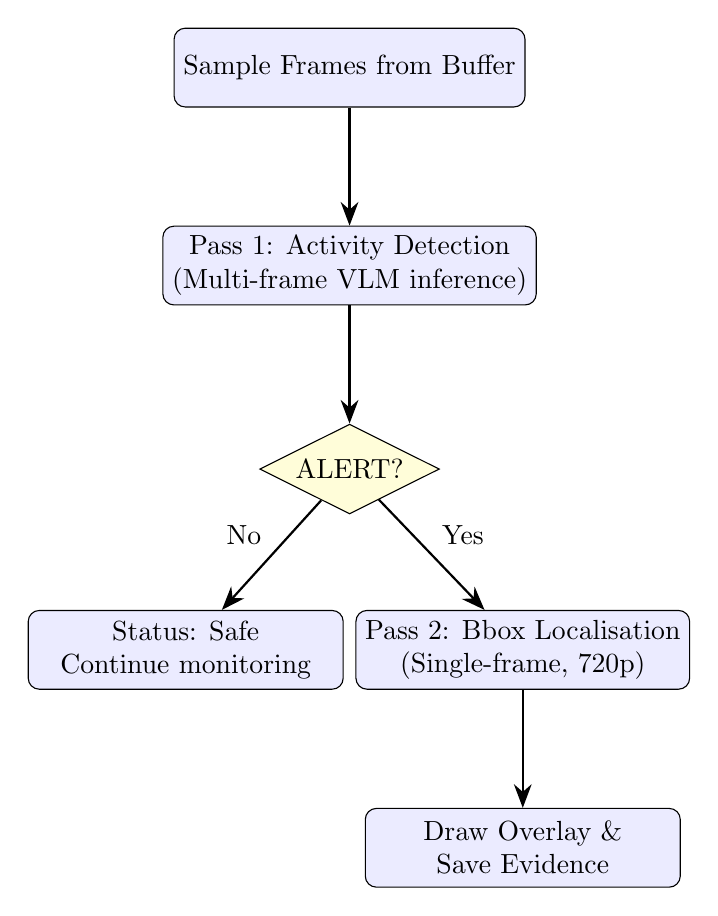
\begin{tikzpicture}[
    node distance=1.5cm,
    block/.style={rectangle, draw, rounded corners, minimum width=4cm, minimum height=1cm, align=center, fill=blue!8},
    decision/.style={diamond, draw, aspect=2, align=center, fill=yellow!15, inner sep=2pt},
    arrow/.style={-{Stealth[length=3mm]}, thick},
]
    \node[block] (sample) {Sample Frames from Buffer};
    \node[block, below=of sample] (pass1) {Pass 1: Activity Detection\\(Multi-frame VLM inference)};
    \node[decision, below=of pass1] (check) {ALERT?};
    \node[block, below left=1.5cm and -0.5cm of check] (safe) {Status: Safe\\Continue monitoring};
    \node[block, below right=1.5cm and -0.5cm of check] (pass2) {Pass 2: Bbox Localisation\\(Single-frame, 720p)};
    \node[block, below=of pass2] (save) {Draw Overlay \&\\Save Evidence};

    \draw[arrow] (sample) -- (pass1);
    \draw[arrow] (pass1) -- (check);
    \draw[arrow] (check) -- node[above left] {No} (safe);
    \draw[arrow] (check) -- node[above right] {Yes} (pass2);
    \draw[arrow] (pass2) -- (save);
\end{tikzpicture}
\caption{Two-pass AI analysis pipeline.}
\label{fig:twopass}
\end{figure}

% ============================================================================
\section{User Interface}
% ============================================================================

The web-based user interface is built with \textbf{Gradio} and is accessible from any browser on the network.

\subsection{Model Loading Panel}

At the top of the interface, a panel allows the user to:

\begin{itemize}[noitemsep]
    \item Select a Qwen VL model from a dropdown list.
    \item Toggle 4-bit quantisation to reduce VRAM requirements.
    \item Click ``Load Model'' to download (on first use) and initialise the model.
    \item View the loading status.
\end{itemize}

Models are downloaded at runtime from HuggingFace Hub and cached locally.

\subsection{Live Context Monitor Tab}

The primary monitoring tab provides:

\begin{itemize}
    \item \textbf{Live Video Feed:} A streaming image display with a status bar overlay showing the latest AI detection result. Safe status is shown in green; alerts in red.
    \item \textbf{Source Selection:} Radio buttons to choose between Camera and Video File input.
    \item \textbf{Configuration Controls:}
    \begin{itemize}[noitemsep]
        \item Camera ID or stream URL text field.
        \item Video file upload widget (MP4, AVI, MOV, MKV).
        \item AI check interval slider (1--10 seconds).
        \item Sampling strategy dropdown (Uniform, Recent Focus, Motion Focus).
        \item Buffer/segment length slider (2--30 seconds).
        \item Frames per segment slider (4--32 frames).
        \item Video mode toggle (experimental temporal encoding).
    \end{itemize}
    \item \textbf{Prompt Editor:} An expandable text area for customising the AI analysis prompt.
    \item \textbf{Start/Stop Controls:} Buttons to begin and halt monitoring.
    \item \textbf{Event Log:} A scrollable text area showing timestamped detection results.
    \item \textbf{Debug Log:} Detailed sampling and inference diagnostics (buffer sizes, frame hashes, model outputs).
    \item \textbf{Debug Options:} Checkboxes to enable debug logging and to save sampled frame contact sheets.
\end{itemize}

\subsection{Manual Analysis Tab}

A secondary tab for one-shot analysis of uploaded images or videos:

\begin{itemize}[noitemsep]
    \item Upload a single image or video file.
    \item Optionally customise the analysis prompt.
    \item Click ``Analyze'' to receive the AI's assessment.
    \item Results are displayed as Markdown text alongside the uploaded image.
\end{itemize}

% ============================================================================
\section{Alert Handling and Evidence Collection}
% ============================================================================

\subsection{Alert Lifecycle}

When the AI detects a prohibited activity:

\begin{enumerate}
    \item The result text (e.g., \texttt{ALERT: Person eating at desk}) is stored in shared state.
    \item The \textbf{alert linger timer} keeps the alert overlay visible for $\text{check\_interval} + 1.5$ seconds, ensuring the user sees it even between AI analysis cycles.
    \item Bounding boxes from Pass~2 are drawn on the live feed as red rectangles with the activity description as a label.
    \item The alert is logged in the Event Log with a timestamp and alarm emoji.
\end{enumerate}

\subsection{Evidence Snapshots}

For every alert, the system automatically saves an \textbf{evidence snapshot}:

\begin{itemize}[noitemsep]
    \item The last frame from the analysed buffer segment is copied.
    \item Bounding boxes and activity labels are burned into the image using OpenCV drawing functions.
    \item The file is saved to \texttt{evidence\_snapshots/} with a filename pattern: \texttt{alert\_YYYYMMDD\_HHMMSS\_<activity>.jpg}.
    \item Activity descriptions are sanitised for filesystem safety.
\end{itemize}

\subsection{Debug Contact Sheets}

When debug frame saving is enabled, sampled frames are stitched into a \textbf{contact sheet} (grid of thumbnails) and saved as a JPEG. This allows visual verification of which frames the AI model received, aiding in prompt and sampling strategy tuning.

% ============================================================================
\section{Configuration and Tuning}
% ============================================================================

\subsection{System Parameters}

The \texttt{Config} dataclass centralises all tunable parameters:

\begin{table}[H]
\centering
\caption{Configurable system parameters.}
\label{tab:config}
\begin{tabular}{@{}llp{6.5cm}@{}}
\toprule
\textbf{Parameter} & \textbf{Default} & \textbf{Description} \\
\midrule
\texttt{buffer\_seconds} & 4 & Duration of the sliding window buffer in seconds. \\
\texttt{sample\_frames} & 8 & Number of frames sampled per AI analysis. \\
\texttt{check\_interval} & 2.0 & Seconds between AI analysis triggers. \\
\texttt{resize\_height} & 480 & Height (px) to which sampled frames are resized. \\
\texttt{display\_max\_width} & 1024 & Maximum display width for the live feed. \\
\texttt{display\_frame\_interval} & 4 & Yield a display frame every $n$ captured frames. \\
\texttt{alert\_linger\_extra} & 1.5 & Extra seconds to keep alert overlays visible. \\
\texttt{max\_log\_entries} & 100 & Maximum event log entries retained. \\
\texttt{max\_debug\_entries} & 200 & Maximum debug log entries retained. \\
\bottomrule
\end{tabular}
\end{table}

\subsection{Runtime Adjustability}

The Gradio UI exposes several parameters for \textbf{runtime adjustment} without restarting the application:

\begin{itemize}[noitemsep]
    \item Buffer/segment length (2--30 seconds).
    \item Number of sampled frames per segment (4--32).
    \item AI check interval (1--10 seconds).
    \item Sampling strategy (Uniform, Recent Focus, Motion Focus).
    \item Analysis prompt (fully editable).
    \item Video mode toggle for temporal encoding.
    \item Debug logging and frame saving toggles.
\end{itemize}

% ============================================================================
\section{Technology Stack}
% ============================================================================

\begin{table}[H]
\centering
\caption{Core technology stack.}
\label{tab:techstack}
\begin{tabular}{@{}lp{8.5cm}@{}}
\toprule
\textbf{Technology} & \textbf{Role} \\
\midrule
Python 3.13/3.14 & Primary programming language. \\
PyTorch (CUDA 13.0) & Deep learning framework with GPU acceleration. \\
HuggingFace Transformers & Model loading, tokenisation, and generation. \\
Qwen-VL-Utils & Vision-language preprocessing utilities for Qwen models. \\
BitsAndBytes & 4-bit NF4 quantisation for reduced VRAM usage. \\
OpenCV & Video capture, frame manipulation, drawing overlays. \\
Gradio & Web-based UI framework with streaming support. \\
Pillow (PIL) & Image format conversion and manipulation. \\
NumPy & Numerical operations, frame sampling, motion scoring. \\
MoviePy / ImageIO & Video I/O utilities. \\
\bottomrule
\end{tabular}
\end{table}

% ============================================================================
\section{Installation and Deployment}
% ============================================================================

\subsection{Prerequisites}

\begin{itemize}[noitemsep]
    \item Python 3.13 or 3.14.
    \item NVIDIA GPU with CUDA support (recommended; CPU fallback available).
    \item Windows operating system (PowerShell install script provided).
    \item A Python virtual environment (\texttt{venv}).
\end{itemize}

\subsection{Installation Steps}

The provided \texttt{install.ps1} PowerShell script automates the setup:

\begin{enumerate}
    \item Activates the virtual environment (or detects an existing active environment).
    \item Installs PyTorch and TorchVision with CUDA 13.0 support from the PyTorch wheel index.
    \item Installs the latest HuggingFace Transformers from the Git repository.
    \item Optionally installs \texttt{llama-cpp-python} with CUDA support for GGUF model inference (experimental). Falls back to CPU build if the CUDA build fails.
    \item Installs all remaining dependencies from \texttt{requirements.txt}.
    \item Removes the \texttt{hf-xet} package to avoid model download issues.
\end{enumerate}

\subsection{Running the Application}

After installation, the application is launched with:

\begin{lstlisting}[language=bash, numbers=none]
python src/app.py
\end{lstlisting}

The Gradio interface starts on \texttt{http://0.0.0.0:7860} and is accessible from any device on the network.

% ============================================================================
\section{Design Decisions and Trade-offs}
% ============================================================================

\subsection{Why Vision-Language Models?}

Traditional computer vision approaches (object detection, pose estimation, action recognition) require task-specific training data and separate models for each activity. VLMs offer:

\begin{itemize}[noitemsep]
    \item \textbf{Zero-shot generalisation:} The model understands activities described in natural language without task-specific fine-tuning.
    \item \textbf{Prompt flexibility:} The set of prohibited activities can be changed instantly by editing the text prompt.
    \item \textbf{Contextual reasoning:} The model can reason about multi-frame temporal context and spatial relationships.
\end{itemize}

\subsection{Two-Pass vs.\ Single-Pass Analysis}

A single-pass approach that simultaneously detects activities and localises offenders was found to be unreliable. Splitting detection (multi-frame, lower resolution) from localisation (single-frame, higher resolution) improves both accuracy and specificity:

\begin{itemize}[noitemsep]
    \item Pass~1 benefits from \textbf{temporal context} across multiple frames.
    \item Pass~2 benefits from \textbf{higher spatial resolution} on a single frame for precise bounding-box regression.
\end{itemize}

\subsection{Thread Safety}

The producer--consumer design with explicit locks ensures that:

\begin{itemize}[noitemsep]
    \item Frame capture runs at full speed without being blocked by AI inference.
    \item AI inference can take variable time without dropping frames.
    \item The UI remains responsive during long inference cycles.
\end{itemize}

\subsection{Quantisation Trade-off}

4-bit NF4 quantisation via BitsAndBytes reduces VRAM usage by approximately 4$\times$ (e.g., a 7B model fits in $\sim$6\,GB instead of $\sim$24\,GB). The trade-off is a small reduction in model accuracy, which is generally acceptable for surveillance activity classification.

% ============================================================================
\section{Limitations and Future Work}
% ============================================================================

\subsection{Current Limitations}

\begin{itemize}
    \item \textbf{Inference Latency:} VLM inference takes 1--5 seconds per analysis cycle depending on the model size and GPU. This introduces a delay between the occurrence of a prohibited activity and its detection.
    \item \textbf{GGUF Support:} GGUF model format support via \texttt{llama-cpp-python} is work-in-progress and requires additional build tools (CMake, Visual Studio Build Tools, CUDA Toolkit).
    \item \textbf{False Positives:} VLMs can occasionally misinterpret benign activities (e.g., drinking water from a bottle vs.\ reaching for a mouse). Prompt engineering helps but does not eliminate this.
    \item \textbf{Single Camera:} The current architecture monitors one video source at a time.
    \item \textbf{Limited Testing:} The manual upload analysis tab is noted as not thoroughly tested.
\end{itemize}

\subsection{Future Enhancements}

\begin{itemize}
    \item \textbf{Multi-camera support} with a unified dashboard.
    \item \textbf{Persistent alert database} with search and filtering.
    \item \textbf{Fine-tuned models} trained on lab surveillance data for improved accuracy.
    \item \textbf{Integration with notification systems} (email, SMS, push notifications).
    \item \textbf{GGUF model support} for CPU-only deployments.
    \item \textbf{Edge deployment} optimisation for embedded devices.
\end{itemize}

% ============================================================================
\section{Conclusion}
% ============================================================================

The \textbf{Qwen Sentinel} system demonstrates a practical application of Vision-Language Models for automated computer lab surveillance. By combining a sliding-window frame buffer with configurable sampling strategies and a two-pass AI analysis pipeline, the system achieves real-time detection and localisation of prohibited activities without any task-specific training. The Gradio-based web interface provides an accessible dashboard for monitoring, configuration, and evidence review. While inference latency and occasional false positives remain challenges, the prompt-driven approach offers unprecedented flexibility in defining and updating the set of monitored activities. The system serves as a foundation for intelligent surveillance solutions that can be extended to multi-camera deployments and integrated with institutional security infrastructure.

% ============================================================================
\appendix
\section{Default Analysis Prompt}
\label{app:prompt}
% ============================================================================

\begin{lstlisting}[language={}, numbers=none, breaklines=true, basicstyle=\ttfamily\small]
Analyze this video clip from a computer lab surveillance camera.
Look at all the shown places and people in the clip. Even in the
background and obscured areas. People may be partially visible,
far away, or in groups. Use the full clip context to understand
their actions. The clip may show multiple people. Determine if
any PROHIBITED activities are occurring.

Check for PROHIBITED activities that require motion context:
1. Running (moving fast across frames)
2. Fighting or Aggressive Physical Contact
3. Eating/Drinking
4. Tampering with equipment
5. Sleeping
6. Phone usage

OUTPUT FORMAT:
If SAFE: 'Status: Safe'
If DANGEROUS: 'ALERT: [Description of activity]'
\end{lstlisting}

% ============================================================================
\section{Strict Mode Suffix (Video Files)}
\label{app:strict}
% ============================================================================

\begin{lstlisting}[language={}, numbers=none, breaklines=true, basicstyle=\ttfamily\small]
STRICT MODE (video file):
If ANY prohibited activity appears in ANY frame, output ALERT.
Do not default to SAFE if uncertain. If motion suggests running
or aggressive contact, alert. If a person appears to eat/drink,
tamper with equipment, phone usage, or sleep, alert. Return
exactly one line in the required format.
\end{lstlisting}

% ============================================================================
\section{Bounding Box Localisation Prompt}
\label{app:bbox}
% ============================================================================

\begin{lstlisting}[language={}, numbers=none, breaklines=true, basicstyle=\ttfamily\small]
This surveillance image contains a person performing a prohibited
activity: {activity}. Look carefully at the ENTIRE image. Locate
the person performing that activity. Return ONLY the bounding box
of that person as [xmin, ymin, xmax, ymax] on a 0-1000 scale
where (0,0) is top-left and (1000,1000) is bottom-right. Return
nothing else.
\end{lstlisting}

\end{document}
